\chapter{从原材料到回收利用}\label{ch:g5:raw-materials-and-recycling}

一个空饮料罐被扔进回收箱，一辆卡车把它运到
分拣中心，机器把它与成千上万个其他罐子
一起压成金属块，熔炉熔化这些金属块，几周后，
金属又以新罐子的形式回到商店货架上。金属最初
从哪里来？为什么要熔化旧罐子，
而不是冶炼新金属？

\begin{recall}
物体是我们能看到、摸到的东西；其材料是指它由
什么制成——木头、金属、玻璃、塑料、纸、布料、石头
（见\cref{ch:g1:materials-around-us}）。\omterm{def:g5:irreversible-changes:chemical-change}{化学变化}中会生成新物质，
且无法简单复原（见\cref{ch:g5:irreversible-changes}）。
\end{recall}

\section{天然材料与人造材料}

\begin{definition}[天然材料与人造材料]\label{def:g5:raw-materials-and-recycling:natural-material}
称\emph{天然材料}\index{天然材料}为
基本保持自然状态、仅经切割或塑形即被使用的材料，如木材、石料、棉、羊毛、皮革；
称\emph{人造材料}\index{人造材料}为人们从自然界的物质出发，
通过改变其性质制成的材料，常伴随加热和\omterm{def:g5:irreversible-changes:chemical-change}{化学变化}，
如玻璃、钢、铝、塑料、纸、
混凝土。
\end{definition}

\begin{example}[两张桌子]\label{ex:g5:raw-materials-and-recycling:tables}
用橡木板制成的桌子用的是\omterm{def:g5:raw-materials-and-recycling:natural-material}{天然材料}：木材只是
经过锯切、刨平和胶合。桌面为玻璃、桌腿为钢的桌子
则用了\omterm{def:g5:raw-materials-and-recycling:natural-material}{人造材料}：玻璃和钢在自然界中都不以
这种形式存在。
\end{example}

\section{原材料}

\begin{definition}[原材料与矿石]\label{def:g5:raw-materials-and-recycling:raw-material}
称\emph{原材料}\index{原材料}为取自自然界、用于制造
材料和物体的物质，如树木、沙子、岩石、原油、
棉、羊毛。从中提取金属的岩石
称为\emph{矿石}\index{矿石}。
\end{definition}

\begin{example}[材料从何而来]\label{ex:g5:raw-materials-and-recycling:from}
\begin{itemize}
  \item 木材和纸来自树木；
  \item 玻璃以沙子为原料，与纯碱和
        石灰石一起强热制得；
  \item 铁和钢来自铁\omterm{def:g5:raw-materials-and-recycling:raw-material}{矿石}，一种红色的岩石；
  \item 铝来自铝土矿，另一种\omterm{def:g5:raw-materials-and-recycling:raw-material}{矿石}；
  \item 大多数塑料来自原油，原油由地下抽取；
  \item 棉来自植物，羊毛来自绵羊。
\end{itemize}
\end{example}

\begin{omfigure}
\begin{minipage}[b]{0.48\linewidth}\centering
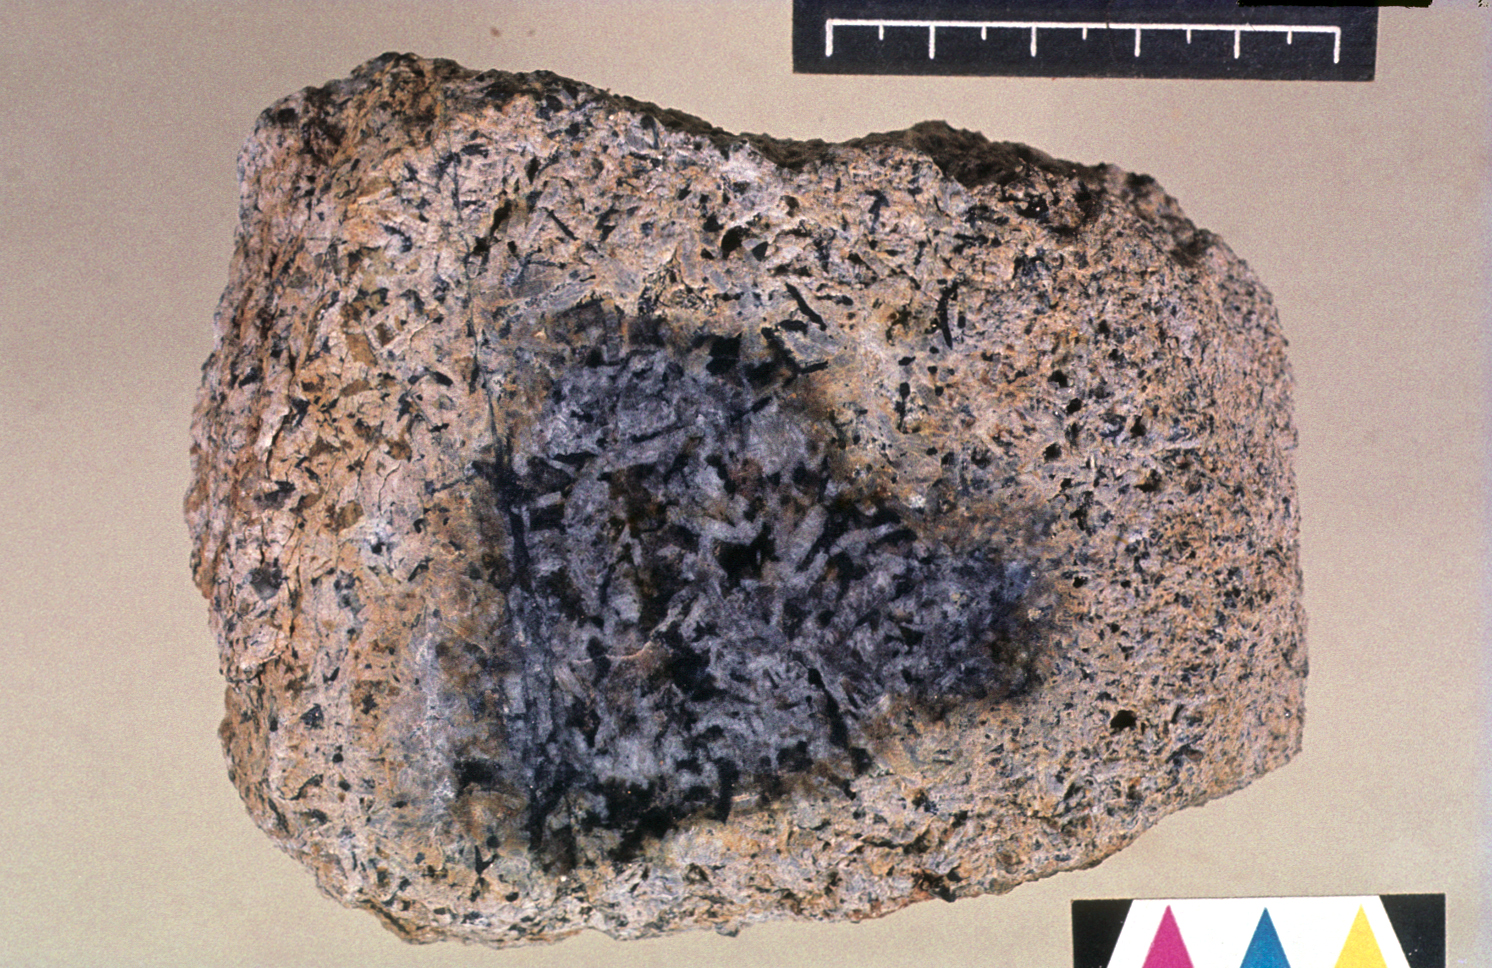
\includegraphics[width=\linewidth,height=4.6cm,keepaspectratio]{images/book1/bauxite.jpg}

{\small 铝土矿，即铝的\omterm{def:g5:raw-materials-and-recycling:raw-material}{矿石}，周围是未风化的
岩石。照片：Werner Schellmann，CC BY-SA 2.5。}
\end{minipage}\hfill
\begin{minipage}[b]{0.48\linewidth}\centering
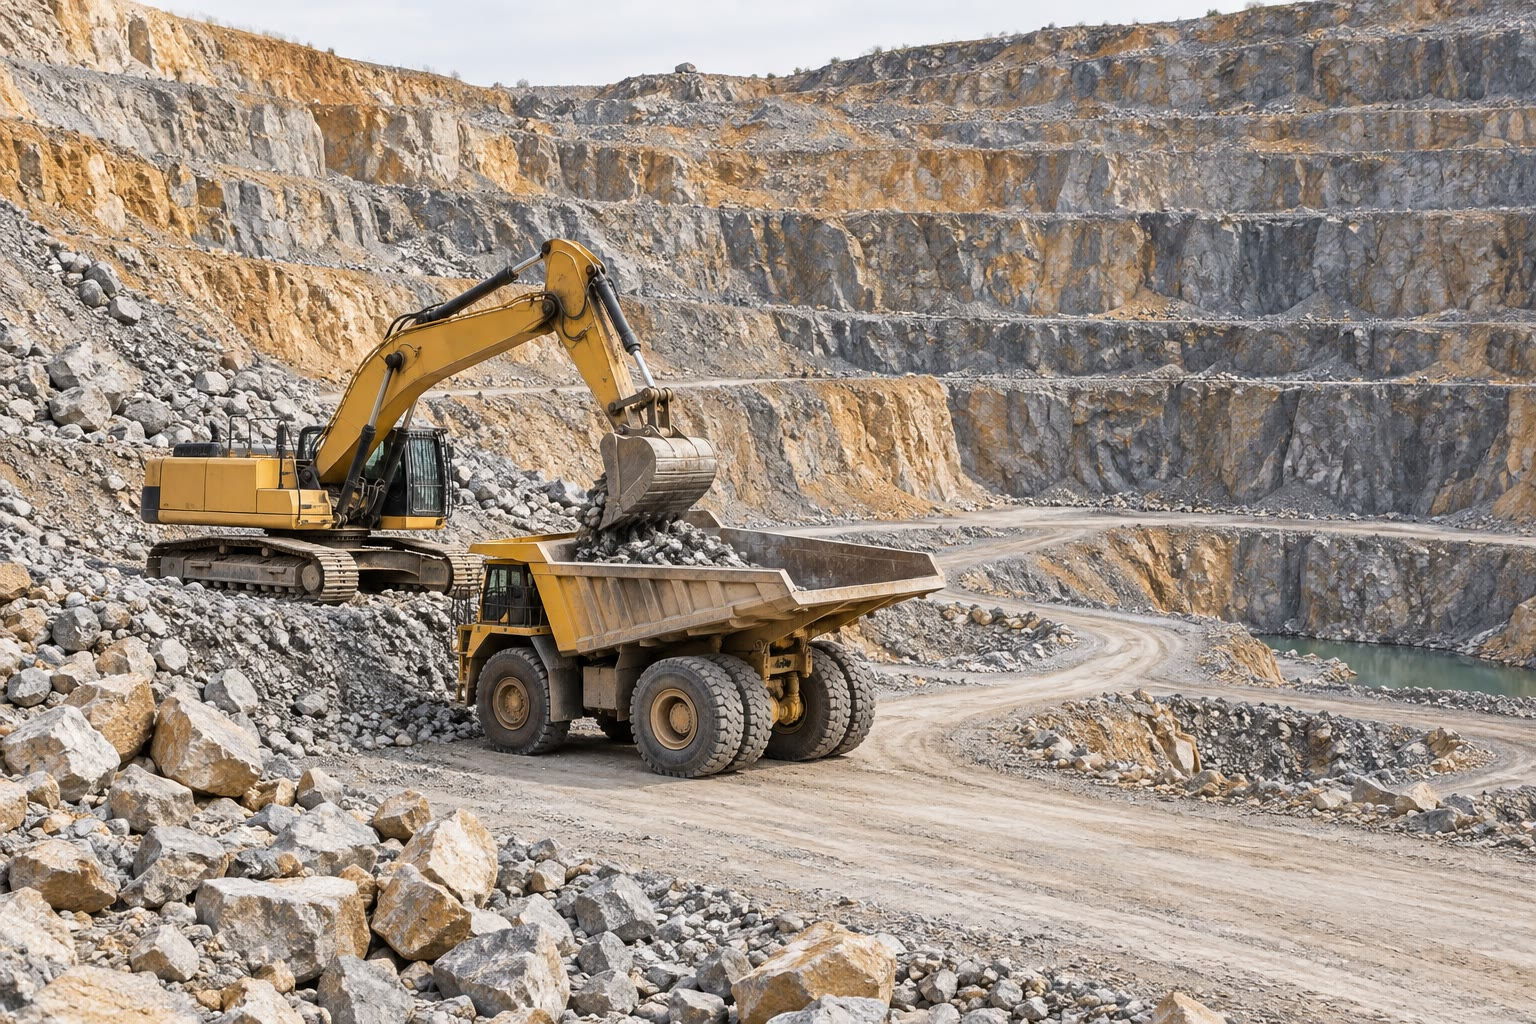
\includegraphics[width=\linewidth,height=4.6cm,keepaspectratio]{images/book1/ai/g5-quarry.jpg}

{\small 采石场：挖出岩石，用作\omterm{def:g5:raw-materials-and-recycling:raw-material}{原材料}。}
\end{minipage}
\end{omfigure}

\begin{omfigure}
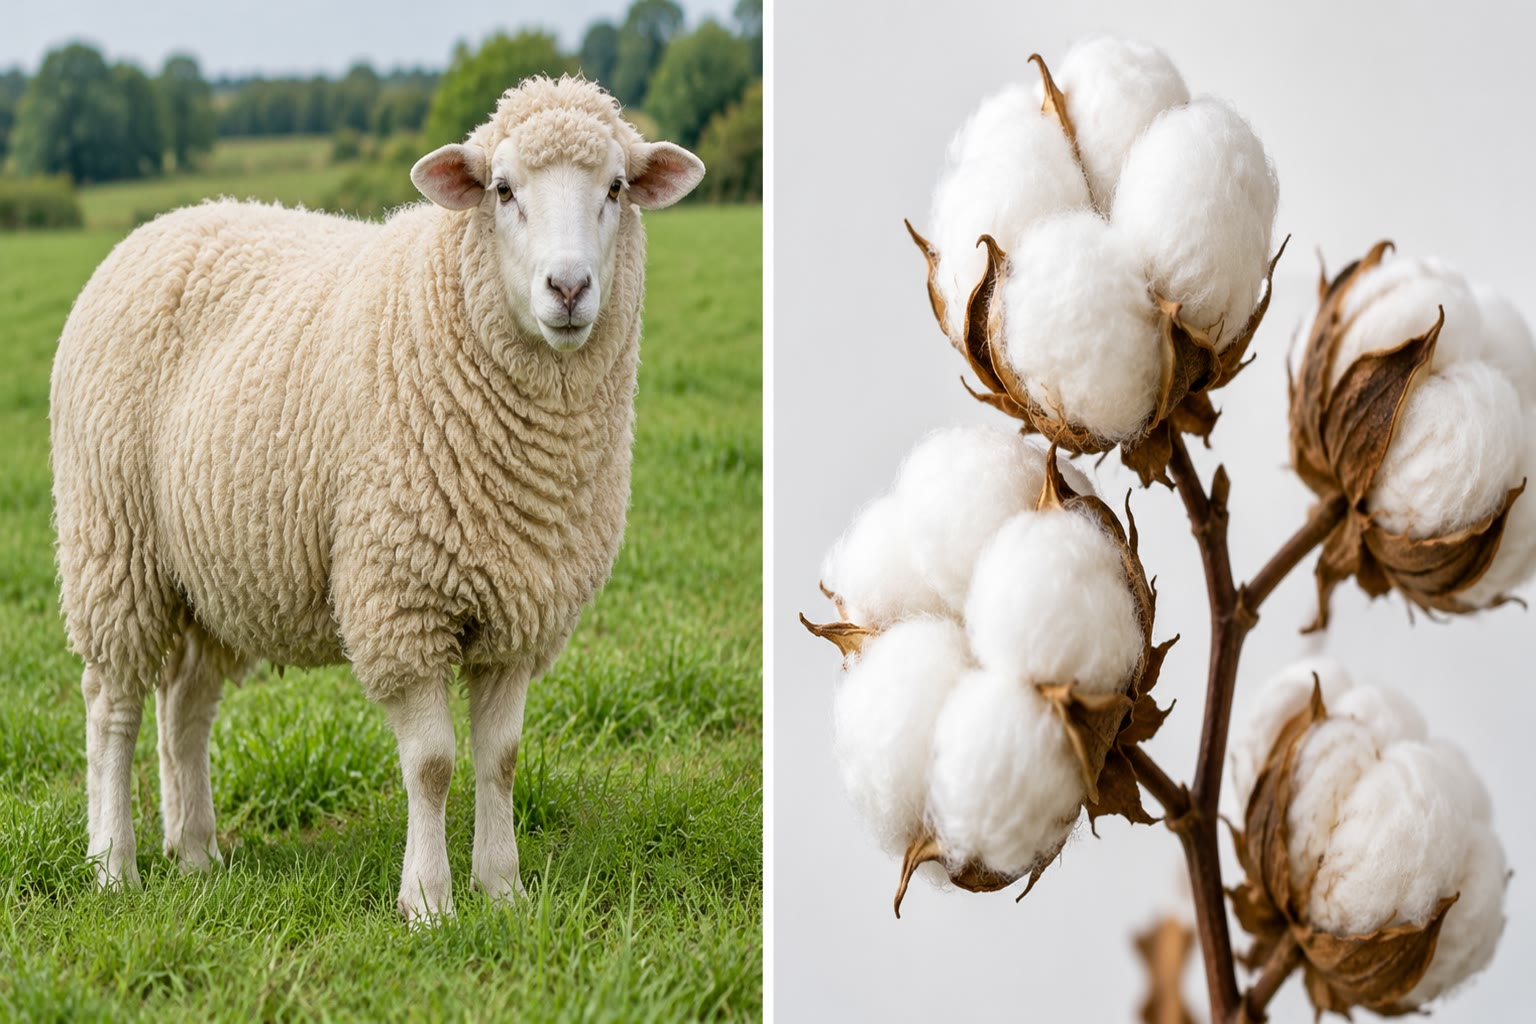
\includegraphics[width=0.6\linewidth]{images/book1/ai/g5-sheep-cotton.jpg}

{\small 取自生物的天然\omterm{def:g5:raw-materials-and-recycling:raw-material}{原材料}：绵羊身上的羊毛、
棉株上采收的棉花。}
\end{omfigure}

\section{从原材料到物体}

\begin{proposition}[制造材料会改变其原材料]\label{prop:g5:raw-materials-and-recycling:change}
将\omterm{def:g5:raw-materials-and-recycling:raw-material}{原材料}制成\omterm{def:g5:raw-materials-and-recycling:natural-material}{人造材料}需要能量——通常是熔炉的热量——
并且通常伴随\omterm{def:g5:irreversible-changes:chemical-change}{化学变化}：沙子变成玻璃，\omterm{def:g5:raw-materials-and-recycling:raw-material}{矿石}变成金属，
原油变成塑料。这些变化不能简单地逆转：玻璃不会
再变回沙子。
\end{proposition}

\begin{example}[一只玻璃瓶的一生]\label{ex:g5:raw-materials-and-recycling:bottle}
沙子、纯碱和压碎的石灰石一起在熔炉中加热，
直至熔化成玻璃。热玻璃被吹制成瓶子的形状。
瓶子装满、售出后被倒空。投入玻璃瓶回收箱后，
它被压碎成小块，再次熔化，吹制成新瓶子：
玻璃被一次又一次地重复利用。
\end{example}

\begin{omfigure}
\begin{tikzpicture}[font=\small,
    box/.style={draw=omDef, fill=omDef!6, rounded corners=2pt, align=center,
      minimum height=0.95cm, text width=2.4cm}]
  \node[box] (r) at (0,2.6) {原材料 \\ （沙子、矿石、原油）};
  \node[box] (m) at (4.0,2.6) {制造 \\ 材料};
  \node[box] (o) at (8.0,2.6) {物体，\\ 已使用};
  \node[box] (w) at (8.0,0) {废弃物};
  \node[box, draw=omProp, fill=omProp!8] (s) at (4.0,0) {分拣与 \\ 回收利用};
  \draw[->, thick, omDef] (r) -- (m);
  \draw[->, thick, omDef] (m) -- (o);
  \draw[->, thick, omDef] (o) -- (w);
  \draw[->, thick, omProp] (w) -- (s);
  \draw[->, thick, omProp] (s) -- (m) node[midway, left, align=right, text=black]
    {重新使用，\\ 代替新的 \\ 原材料};
  \draw[->, thick, black!45, dashed] (w.east) -- ++(1.4,0) node[right, align=left,
    text=black] {丢弃：\\ 填埋};
\end{tikzpicture}

{\small 材料的一生。橙色循环表示\omterm{def:g5:raw-materials-and-recycling:recycling}{回收利用}：
旧物体的材料代替新的原料。}
\end{omfigure}

\section{分拣与回收利用}

\begin{definition}[回收利用]\label{def:g5:raw-materials-and-recycling:recycling}
\emph{回收利用}\index{回收利用}是收集用过的物体，
并对其材料进行处理，使其能够用来制造新的物体，
而不是被丢弃。
\end{definition}

\begin{proposition}[为什么要回收]\label{prop:g5:raw-materials-and-recycling:why}
% ledger: al:energy-primary, al:energy-recycled (8.3 / 186 = about 1/22)
\omterm{def:g5:raw-materials-and-recycling:recycling}{回收利用}可以节省原料，这些原料无需从
地下挖掘，而且通常还能节约能量。用旧易拉罐制造铝，
所需能量只约为用铝土矿制造铝所需能量的二十分之一。
这也意味着填埋场中的废弃物减少。
\end{proposition}

\begin{method}[分拣废弃物以便回收利用]\label{met:g5:raw-materials-and-recycling:sort}
\omterm{def:g5:raw-materials-and-recycling:recycling}{回收利用}从分拣开始，无论废弃物在哪里被丢弃：
\begin{enumerate}
  \item 玻璃瓶和广口瓶放入同一个垃圾桶；
  \item 金属罐、纸和纸板，以及塑料瓶，放入镇上为它们提供的
        垃圾桶中（垃圾桶的颜色
        因地而异）；
  \item 其余废弃物中无法\omterm{def:g5:raw-materials-and-recycling:recycling}{回收利用}的部分。
\end{enumerate}
每种材料都有各自的回收方式，因此每个垃圾桶只能装
它所对应的材料。
\end{method}

\begin{omfigure}
\begin{tikzpicture}[font=\small]
  \foreach \k/\t/\bc in {0/玻璃/green!50!black, 1/{金属罐}/gray,
                        2/{纸和纸板}/omDef, 3/{塑料瓶}/orange!80!black} {
    \begin{scope}[xshift=\k*3.4cm]
      \fill[\bc!18, draw=\bc, line width=0.8pt] (-1,0) -- (1,0) -- (1.15,2.0)
        -- (-1.15,2.0) -- cycle;
      \fill[\bc!45, draw=\bc] (-1.25,2.0) rectangle (1.25,2.3);
      \node[anchor=north, align=center] at (0,-0.15) {\t};
    \end{scope}
  }
  % glass: a bottle
  \fill[green!40!black!60] (-0.2,0.3) rectangle (0.2,1.2);
  \fill[green!40!black!60] (-0.07,1.2) rectangle (0.07,1.6);
  % metal: a can
  \begin{scope}[xshift=3.4cm]
    \fill[black!25, draw=black!55] (-0.3,0.3) rectangle (0.3,1.3);
  \end{scope}
  % paper: a box and a sheet
  \begin{scope}[xshift=6.8cm]
    \fill[brown!25, draw=brown!60] (-0.6,0.3) rectangle (0.1,1.0);
    \fill[white, draw=black!40] (0.2,0.3) rectangle (0.65,1.3);
  \end{scope}
  % plastic: a bottle
  \begin{scope}[xshift=10.2cm]
    \fill[cyan!20, draw=cyan!50!black] (-0.25,0.3) rectangle (0.25,1.3);
    \fill[cyan!20, draw=cyan!50!black] (-0.1,1.3) rectangle (0.1,1.6);
  \end{scope}
\end{tikzpicture}

{\small 四个分类垃圾桶，每种材料一个。（真实垃圾桶的颜色
各城镇之间有所不同。）}
\end{omfigure}

\begin{omfigure}
\begin{minipage}[t]{0.48\linewidth}\centering
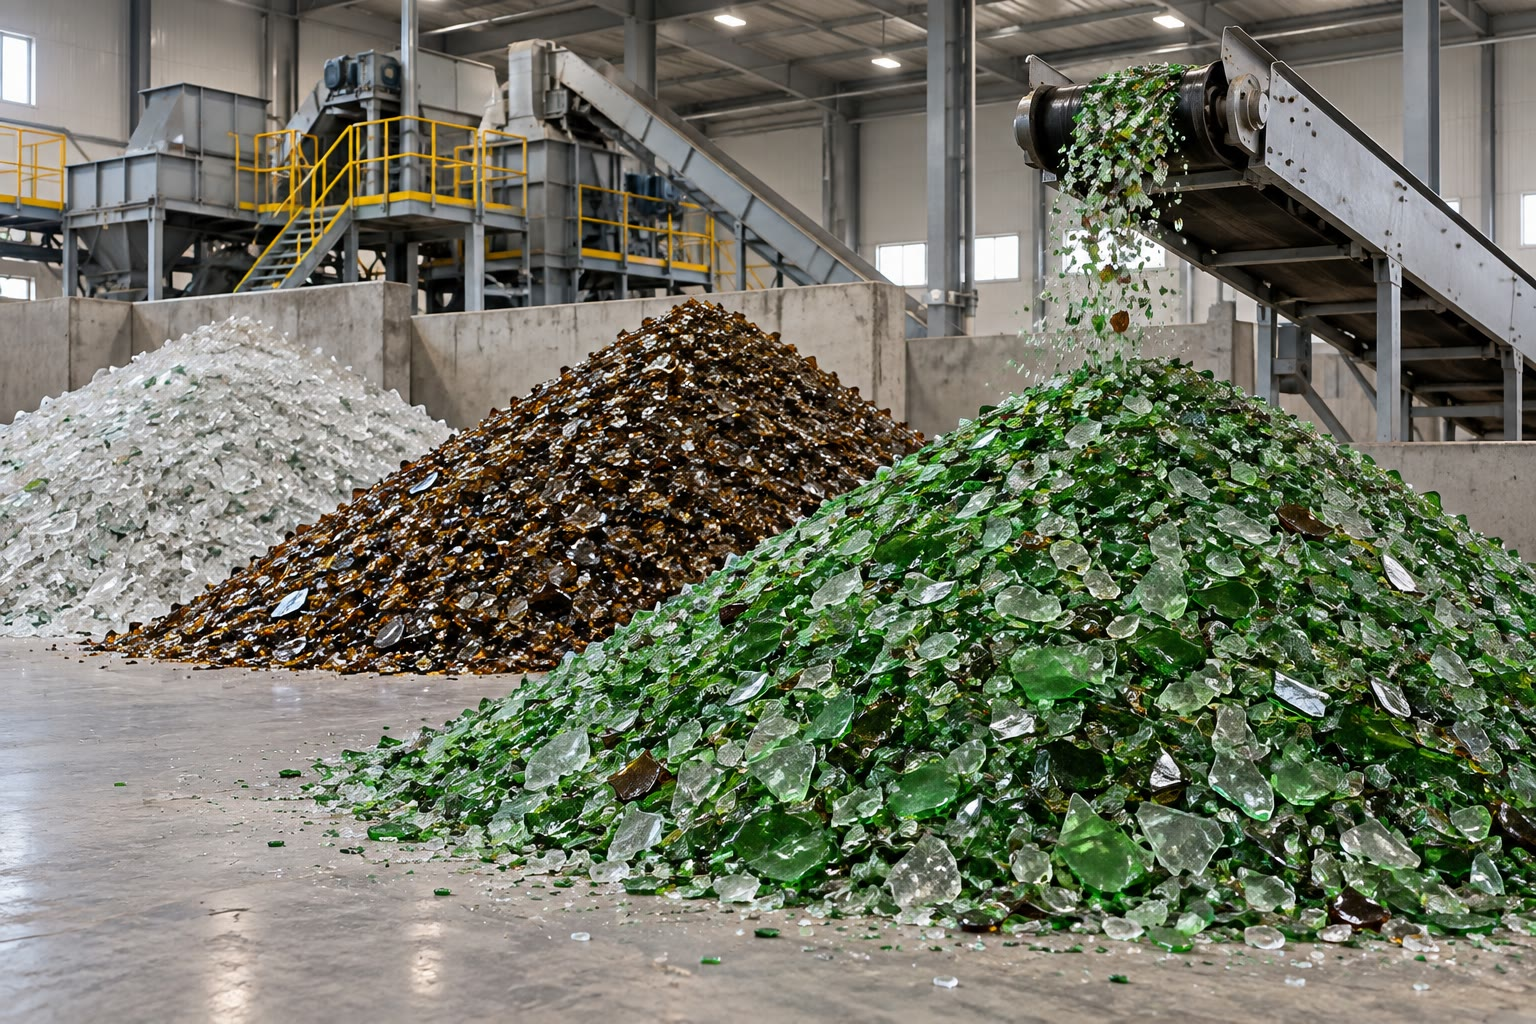
\includegraphics[width=\linewidth,height=4.6cm,keepaspectratio]{images/book1/ai/g5-glass-cullet.jpg}

{\small 回收厂中待熔化的碎玻璃。}
\end{minipage}\hfill
\begin{minipage}[t]{0.48\linewidth}\centering
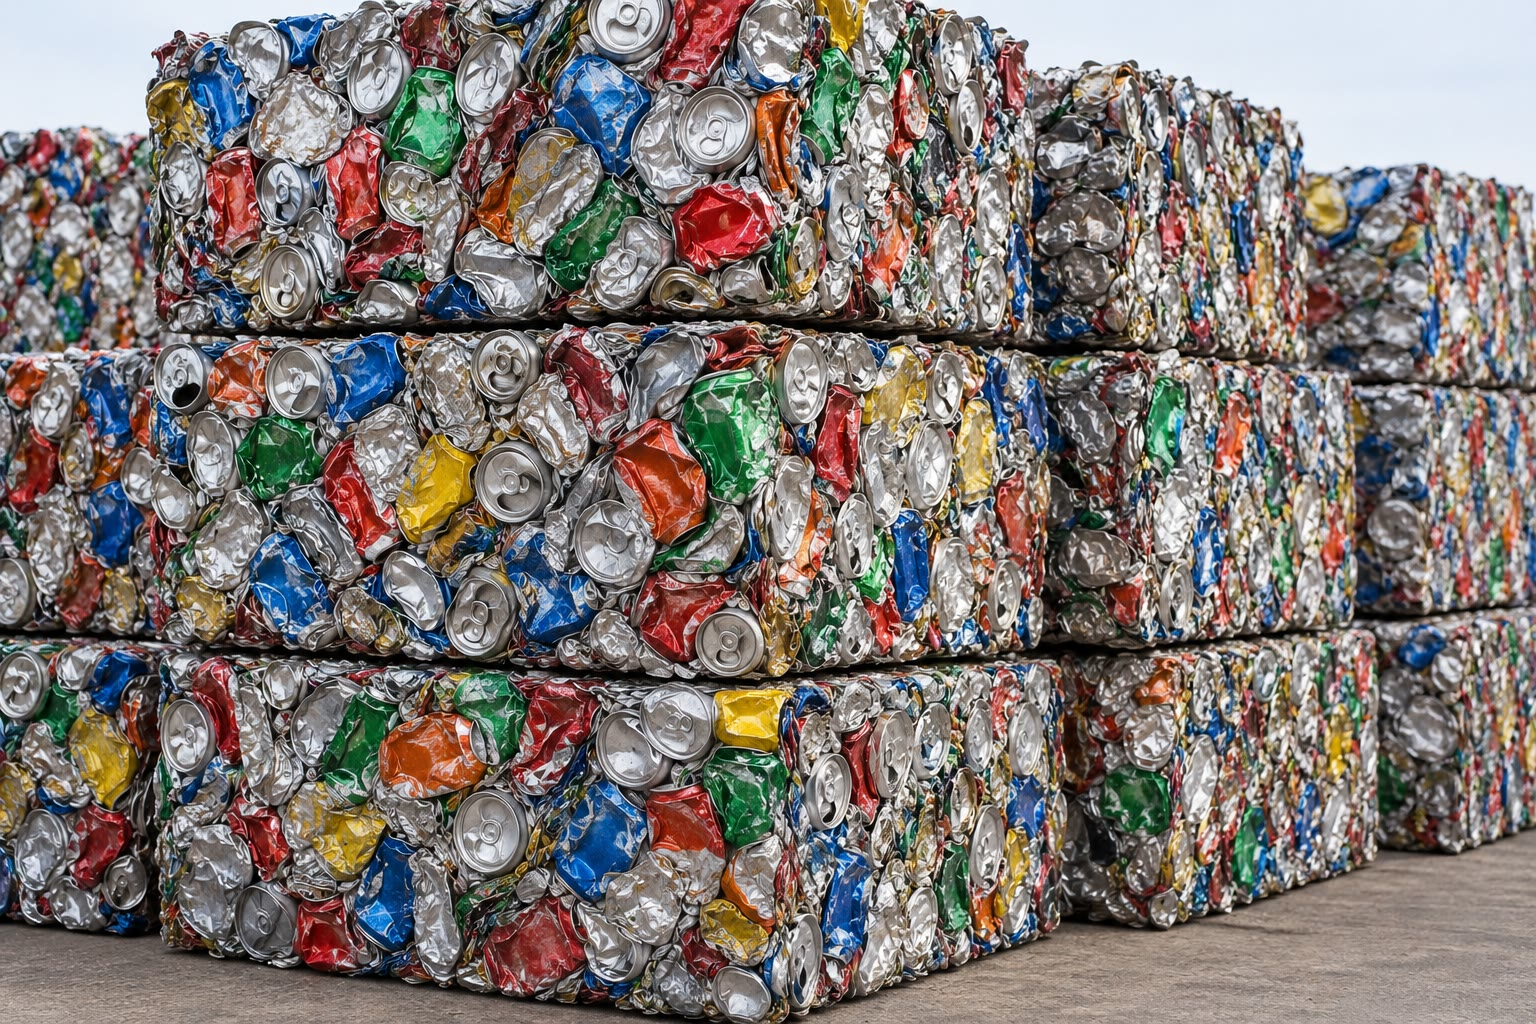
\includegraphics[width=\linewidth,height=4.6cm,keepaspectratio]{images/book1/ai/g5-can-bales.jpg}

{\small 压扁后打包的铝制易拉罐。}
\end{minipage}
\end{omfigure}

\section{废弃物与资源}

\begin{definition}[资源]\label{def:g5:raw-materials-and-recycling:resource}
\emph{资源}\index{资源}是指一切取自自然界、人们所使用的东西：
水、木材、\omterm{def:g5:raw-materials-and-recycling:raw-material}{矿石}、石油、沙子。\emph{可再生
资源}\index{可再生资源}是指在人的一生中能够自行再生或
恢复的资源，例如经过补种的森林中的木材，或绵羊身上的羊毛。
\omterm{def:g5:raw-materials-and-recycling:raw-material}{矿石}和原油不可再生：一旦挖出
并被使用，就不复存在了。
\end{definition}

\begin{proposition}[减少、再利用、回收利用]\label{prop:g5:raw-materials-and-recycling:three}
为使\omterm{def:g5:raw-materials-and-recycling:resource}{资源}更持久，人们可以按以下顺序进行：
\begin{enumerate}
  \item \textbf{减少}：少用物体，例如少用
        包装物；
  \item \textbf{再利用}：再次使用同一物体，例如把玻璃罐
        重新装满，或把袋子带回商店；
  \item \textbf{\omterm{def:g5:raw-materials-and-recycling:recycling}{回收利用}}：把材料制成新的物体。
\end{enumerate}
\omterm{def:g5:raw-materials-and-recycling:recycling}{回收利用}排在最后，因为它仍需要能量和机器；
最好的废弃物，是永远不被产生的那一种。
\end{proposition}

\section{练习}

\begin{exercise}[$\star$]\label{exo:g5:raw-materials-and-recycling:1}
\omterm{def:g5:raw-materials-and-recycling:natural-material}{天然材料}还是\omterm{def:g5:raw-materials-and-recycling:natural-material}{人造材料}？木材、玻璃、羊毛、钢、塑料、石头。
\end{exercise}

\begin{exercise}[$\star$]\label{exo:g5:raw-materials-and-recycling:2}
说出下列物品的原料：一张纸、一个玻璃罐、一件棉质
T恤、一个塑料瓶。
\end{exercise}

\begin{exercise}[$\star$]\label{exo:g5:raw-materials-and-recycling:3}
什么是\omterm{def:g5:raw-materials-and-recycling:raw-material}{矿石}？写出铝的\omterm{def:g5:raw-materials-and-recycling:raw-material}{矿石}名称。
\end{exercise}

\begin{exercise}[$\star$]\label{exo:g5:raw-materials-and-recycling:4}
下列物品应放入哪个回收箱：空果酱瓶、报纸、饮料罐、
塑料水瓶？
\end{exercise}

\begin{exercise}[$\star$]\label{exo:g5:raw-materials-and-recycling:5}
观察材料生命周期图，橙色循环
箭头代替的是什么？
\end{exercise}

\begin{exercise}[$\star$]\label{exo:g5:raw-materials-and-recycling:6}
判断下列物质哪些是可再生的：木材、原油、羊毛、铁\omterm{def:g5:raw-materials-and-recycling:raw-material}{矿石}、棉花？
\end{exercise}

\begin{exercise}[$\star$]\label{exo:g5:raw-materials-and-recycling:7}
为什么把玻璃冷却后不能变回沙子？
\end{exercise}

\begin{exercise}[$\star$]\label{exo:g5:raw-materials-and-recycling:8}
请各举一种方法：减少、再利用、\omterm{def:g5:raw-materials-and-recycling:recycling}{回收利用}各一种。
\end{exercise}

\begin{exercise}[$\star$]\label{exo:g5:raw-materials-and-recycling:9}
为什么玻璃回收箱只能放玻璃？
\end{exercise}

\begin{exercise}[$\star\star$]\label{exo:g5:raw-materials-and-recycling:10}
用旧罐头盒制铝所需的能量，约为用铝土矿制铝所需能量的二十分之一。
某工厂用铝土矿制作一批铝需要 20 单位能量。
若改用旧罐头盒制作同样一批铝，
大约需要多少单位能量？
\end{exercise}

\begin{exercise}[$\star\star$]\label{exo:g5:raw-materials-and-recycling:11}
为什么“减少”排在“\omterm{def:g5:raw-materials-and-recycling:recycling}{回收利用}”前面？
\end{exercise}
